%%%%%%%%%%%%%%%%%%%%%%%%%%%%%%%%%%%%%%%%%%%%%%%%%%%%%%%%%%%%%%%%%%%%%%%%%%%%%%%

\chapter{CASE STUDY: HURRICANE BERYL}
\label{ch:beryl}

This chapter explores the results of implementing cold pool parameterization in the latest Brazilian numerical weather and climate prediction model. It focuses on its performance in forecasting hurricane trajectory, intensity, and rainfall. It specifically focuses on the case study of Hurricane Beryl, which occurred in June and July 2024 in the North Atlantic Ocean. Following a brief event description as an introduction, the chapter describes the data utilized, the numerical model employed, and the evaluation framework established. Finally, the findings are presented and discussed.
% VISTO

\section{Event description - hurricane Beryl}

\pagebreak


% ======================================================================================= %

\section{Results and analysis of hurricane Beryl}

In this section, we will present the results in alignment with the established workflow and engage in a discussion regarding the questions outlined in Table~\ref{tab:questions}. The subsequent subsections will detail the trajectory, intensity, and rainfall analyses. To conclude, we will provide a summary discussion highlighting the key outcomes of the model and evaluating the overall performance of MONAN in comparison with ERA5.

By the workflow sequence, we will begin by addressing the selection process. Table~\ref{tab:experiments_long} illustrates all the experiments that were conducted.

\begin{center}
\captionof{table}{All Performed Experiments} \label{tab:experiments_long}
\end{center}

\begin{longtable}{m{3cm} m{8cm} m{3.5cm}}
\textbf{Experiment} & \textbf{Description} & \textbf{ID} \\
\hline
\endfirsthead

\textbf{Experiment} & \textbf{Description} & \textbf{ID} \\
\hline
\endhead

\multicolumn{3}{r}{\textit{Table continued on next page}} \\
\endfoot

\hline
\endlastfoot

Cold Pool Effect & Turn on and off the cold pool parameterization scheme & \makecell[l]{CP-ON\\CP-OFF (Control)} \\
\hline
Initial Condition Day & Compares the effect of four initial conditions, June 29, 1st July, July 2nd (noon) and July 3rd. & \makecell[l]{CP-29\\CP-01\\CP-02T12\\CP-03 (Control)} \\
\hline
Cold Pool Lifetime & Compares the effect of cold pool lifetime being 1h, 2h (default), 3h, and 6h & \makecell[l]{CP-1H\\CP-2H (Control)\\CP-3H\\CP-6H} \\
\hline
Maximum Downdraft Height & Compares the effect of the maximum downdraft height, being 0.25, 0.35, and 0.50 & \makecell[l]{CP-D025\\CP-D035 (Control)\\CP-D050} \\
\hline
Resolution Experiment & Evaluates the resolution effect on the results, degrading it into 60 km and enhancing it into 15 km & \makecell[l]{CP-15km\\CP-30km (Control)\\CP-60km} \\
\hline
Type of Initial Condition & Changes the type of initial condition to be from the GFS model & \makecell[l]{CP-ERA5 (Control)\\CP-GFS} \\
\hline
Best Configuration Test & A run with two changes inside the cold pool parameters & \makecell[l]{CP-1HD050\\CP-1HD05015km} \\
\end{longtable}

\begin{center}
Source: Made by the author (2025).
\end{center}

The “ID” column serves as a reference for the names of the experiments. It is important to note that in the results, CP-ON represents the default configuration. In the sensitivity analyses conducted, the default values are specified in the labels. For instance, in the “Resolution Experiment”, the default configuration is set to a grid of 30 km (CP-30km), which is then changed to 60 km (CP-60km) and 15 km (CP-15km). To clarify, the following table emphasizes the default parameters:

\begin{center}
\captionof{table}{Default values for the cold pool parameterization scheme} \label{tab:cp_default}
\begin{tabular}{m{5.5cm} m{6cm}}
\textbf{Parameter} & \textbf{Default Value} \\
\hline
Initial Condition Day & July 3rd (00 UTC), 2024 \\
Cold Pool Lifetime & 2 h \\
Maximum Downdraft Height & 0.35 \\
Resolution Experiment & 30 km grid \\
Type of Initial Condition & Coming from ERA5 \\
\end{tabular}
\vspace{0.5em}

Source: Made by the author, 2025.
\end{center}


We investigate the impact of cold pools by enabling (CP-ON) and disabling (CP-OFF) the parameterization, with CP-OFF serving as the control experiment in this case. In the subsequent rows, we conducted a sensitivity analysis on the parameters within the parameterization. Now our control experiment is the CP-ON configuration, with the Table~\ref{tab:cp_default} parameters. For the “Initial Condition Day” experiment, we varied the initial integration times: June 29 (00 UTC), 2024; July 1 (00 UTC), 2024; and July 2 (12 UTC), 2024 - comparing them with the default time. These periods were selected because they correspond to key moments in the storm’s evolution: shortly after HB was classified as a tropical storm, one day before it reached Category 5, and the day it reached Category 5, respectively.

The “Cold Pool Lifetime” was adjusted from the default to durations of 1 hour, 3 hours, and 6 hours. The height of the mass flux above the surface is described by a parabolic function, and the coefficient of this function can be manipulated to alter the maximum height, with lower (higher) values indicating proximity (distance) to the surface. The “Type of Initial Condition” was switched from ERA5 to GFS, both initialized on July 3 (00 UTC), 2024.

During the computation of the initial 13 experiments, we observed that setting the cold pool lifetime to 1 hour and adjusting the maximum downdraft height coefficient to 0.5 resulted in lower errors in the initial results. Consequently, we conducted the “Best Configuration Test” with these parameter adjustments and repeated this configuration at 15 km, bringing the total number of experiments to 15. The reference data here is the best track dataset, and hereafter this dataset will be referenced as “NOAA”. 

Keeping this in mind, Figure~\ref{fig:all_tracks_before} shows all the trajectories for the 15 experiments, plus ERA5 and the reference best-track dataset.

\begin{figure}[!htb]
    \centering
    \caption{Comparison of Storm Tracks Across All 15 Experiments} % Título acima da figura
    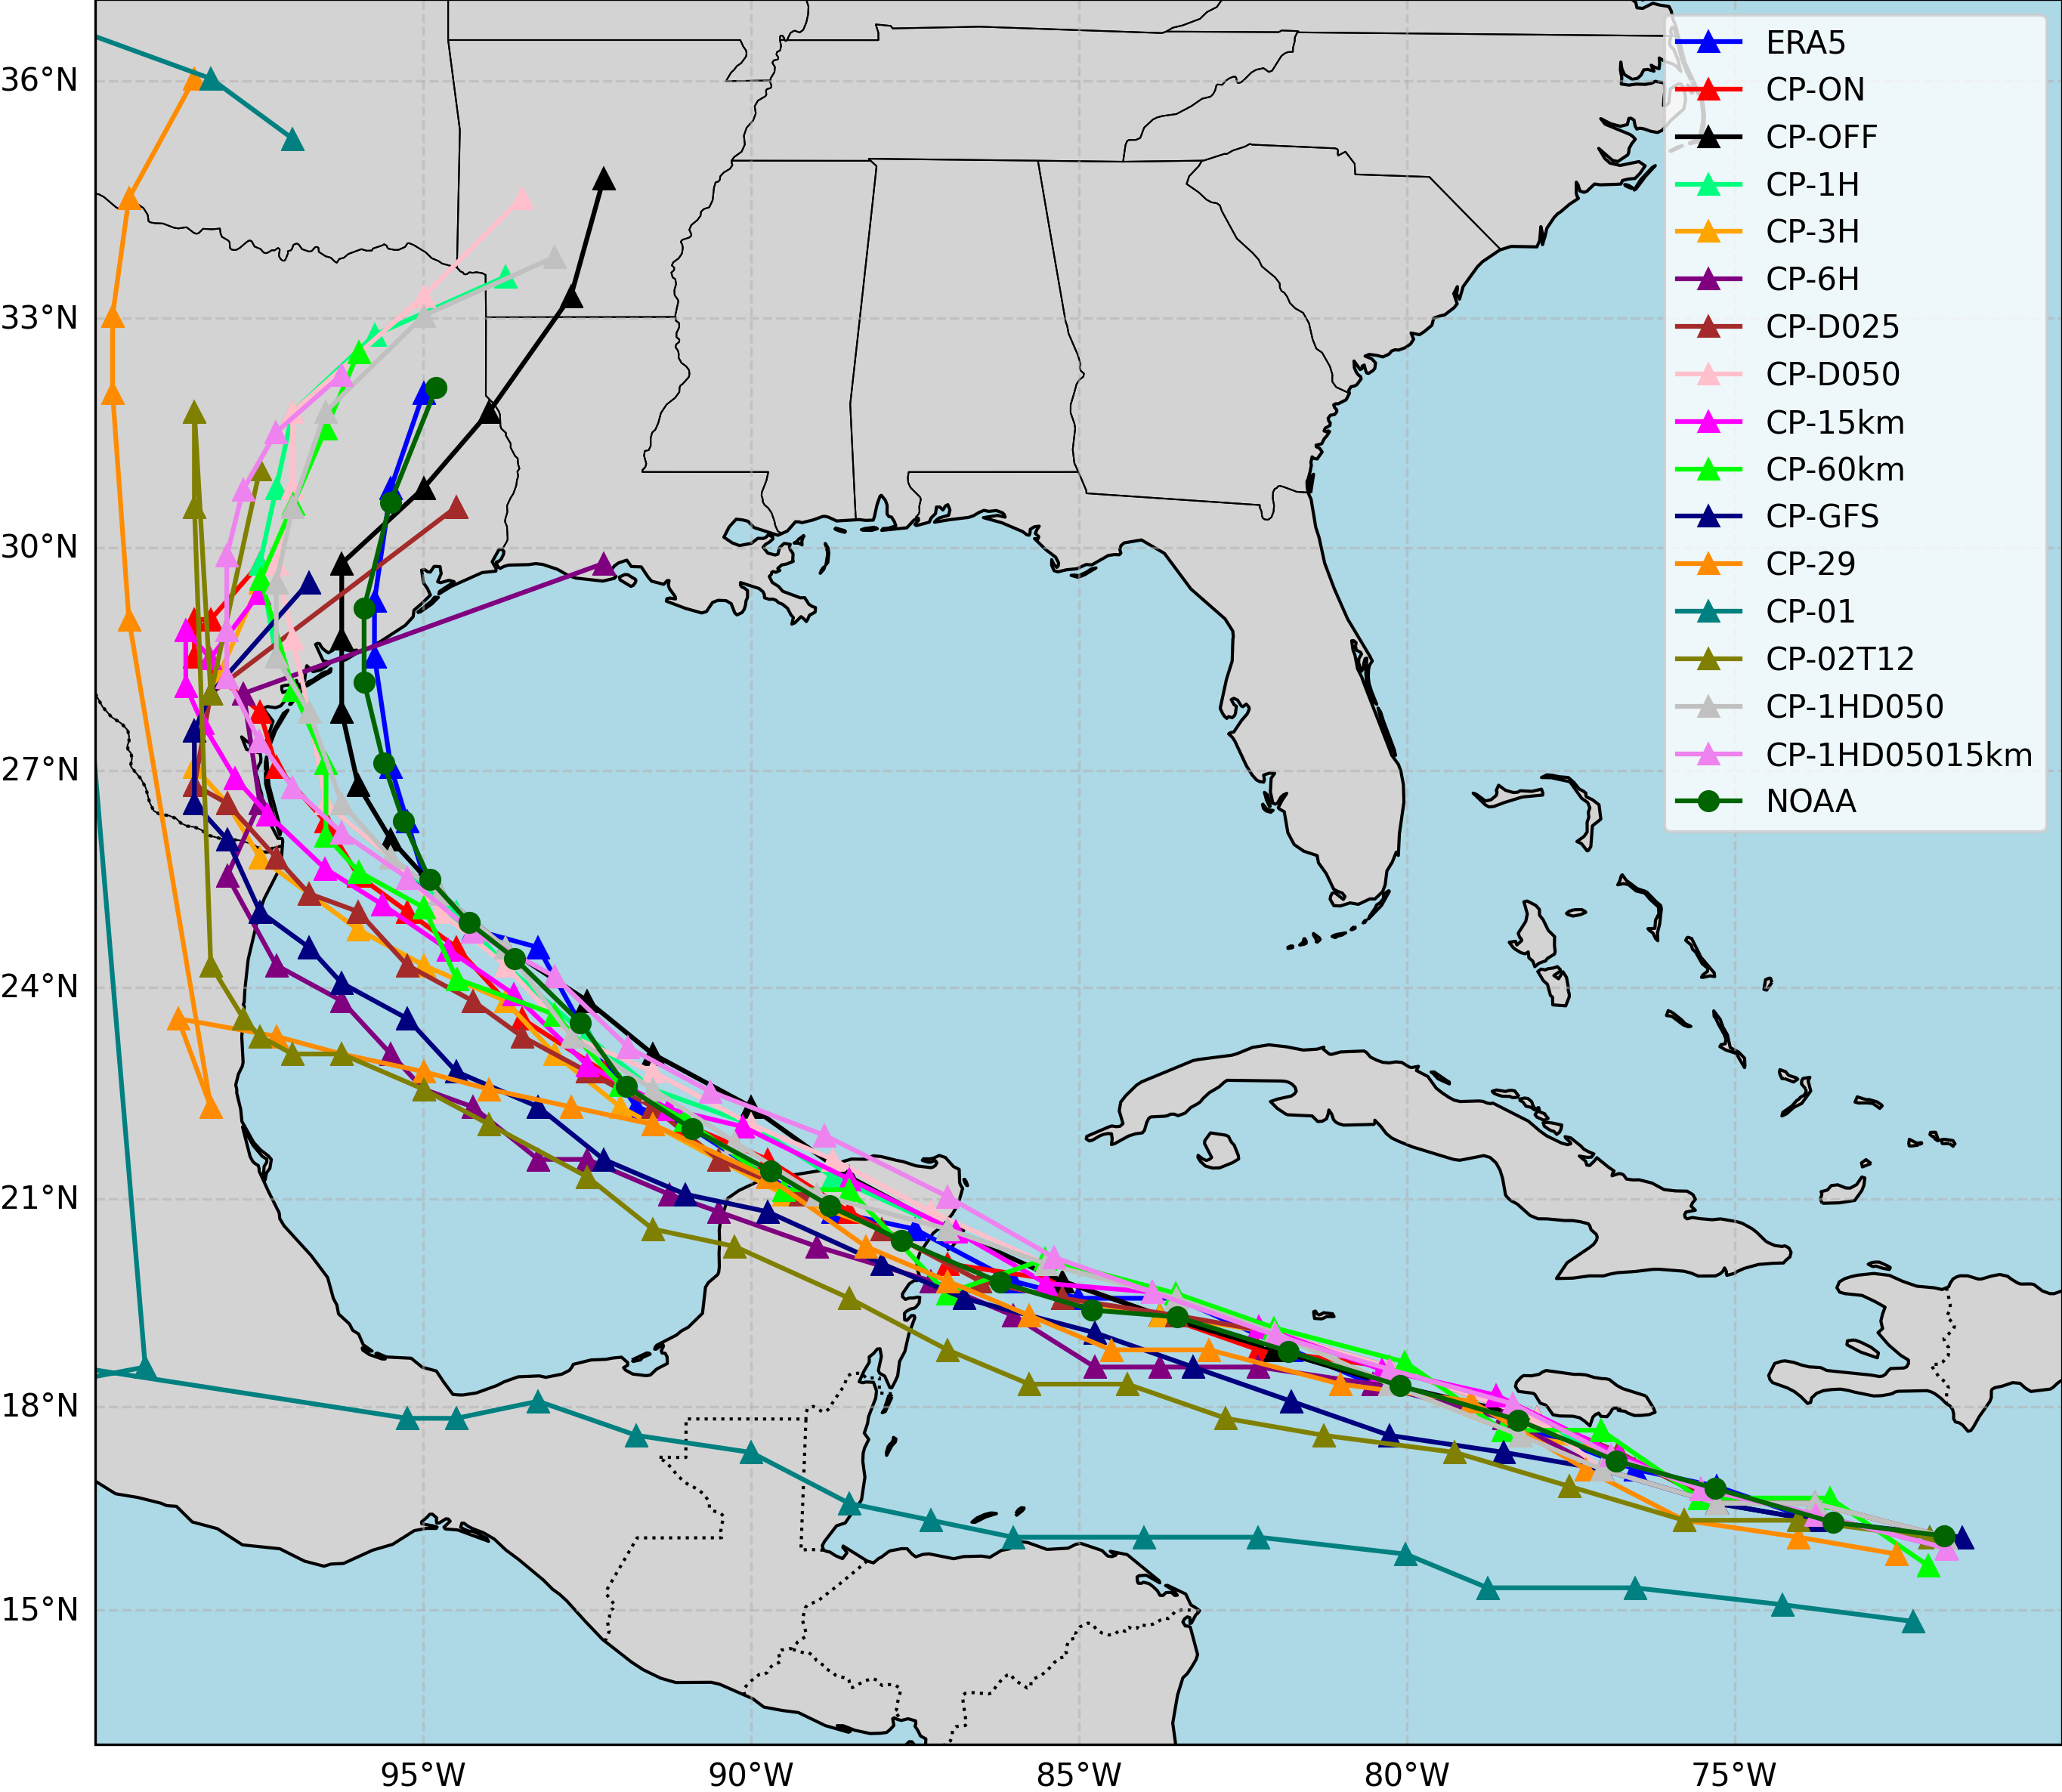
\includegraphics[width=\textwidth]{docs/figuras/findings/ALL_tracks.png} % Substitua pelo caminho e extensão correta
    \vspace{0.5em}
    
    Source: Made by the author (2025). % Fonte abaixo da imagem
    \label{fig:all_tracks_before} % Label para referenciar no texto
\end{figure}

As one can see in Figure~\ref{fig:all_tracks_before}, the numerous experiments clutter the scene and make visual comparison difficult. But one could notice the deviation of CP-6H and CP-01, which could be candidates to be withdrawn. To better visualize the difference between the trajectories, the distance between each trajectory and the reference data (NOAA’s best track) was computed and shown in Figure~\ref{fig:panel_errors_before}.

\begin{figure}[!htb]
    \centering
    \caption{Errors (distance) between the trajectories} % Título acima da figura
    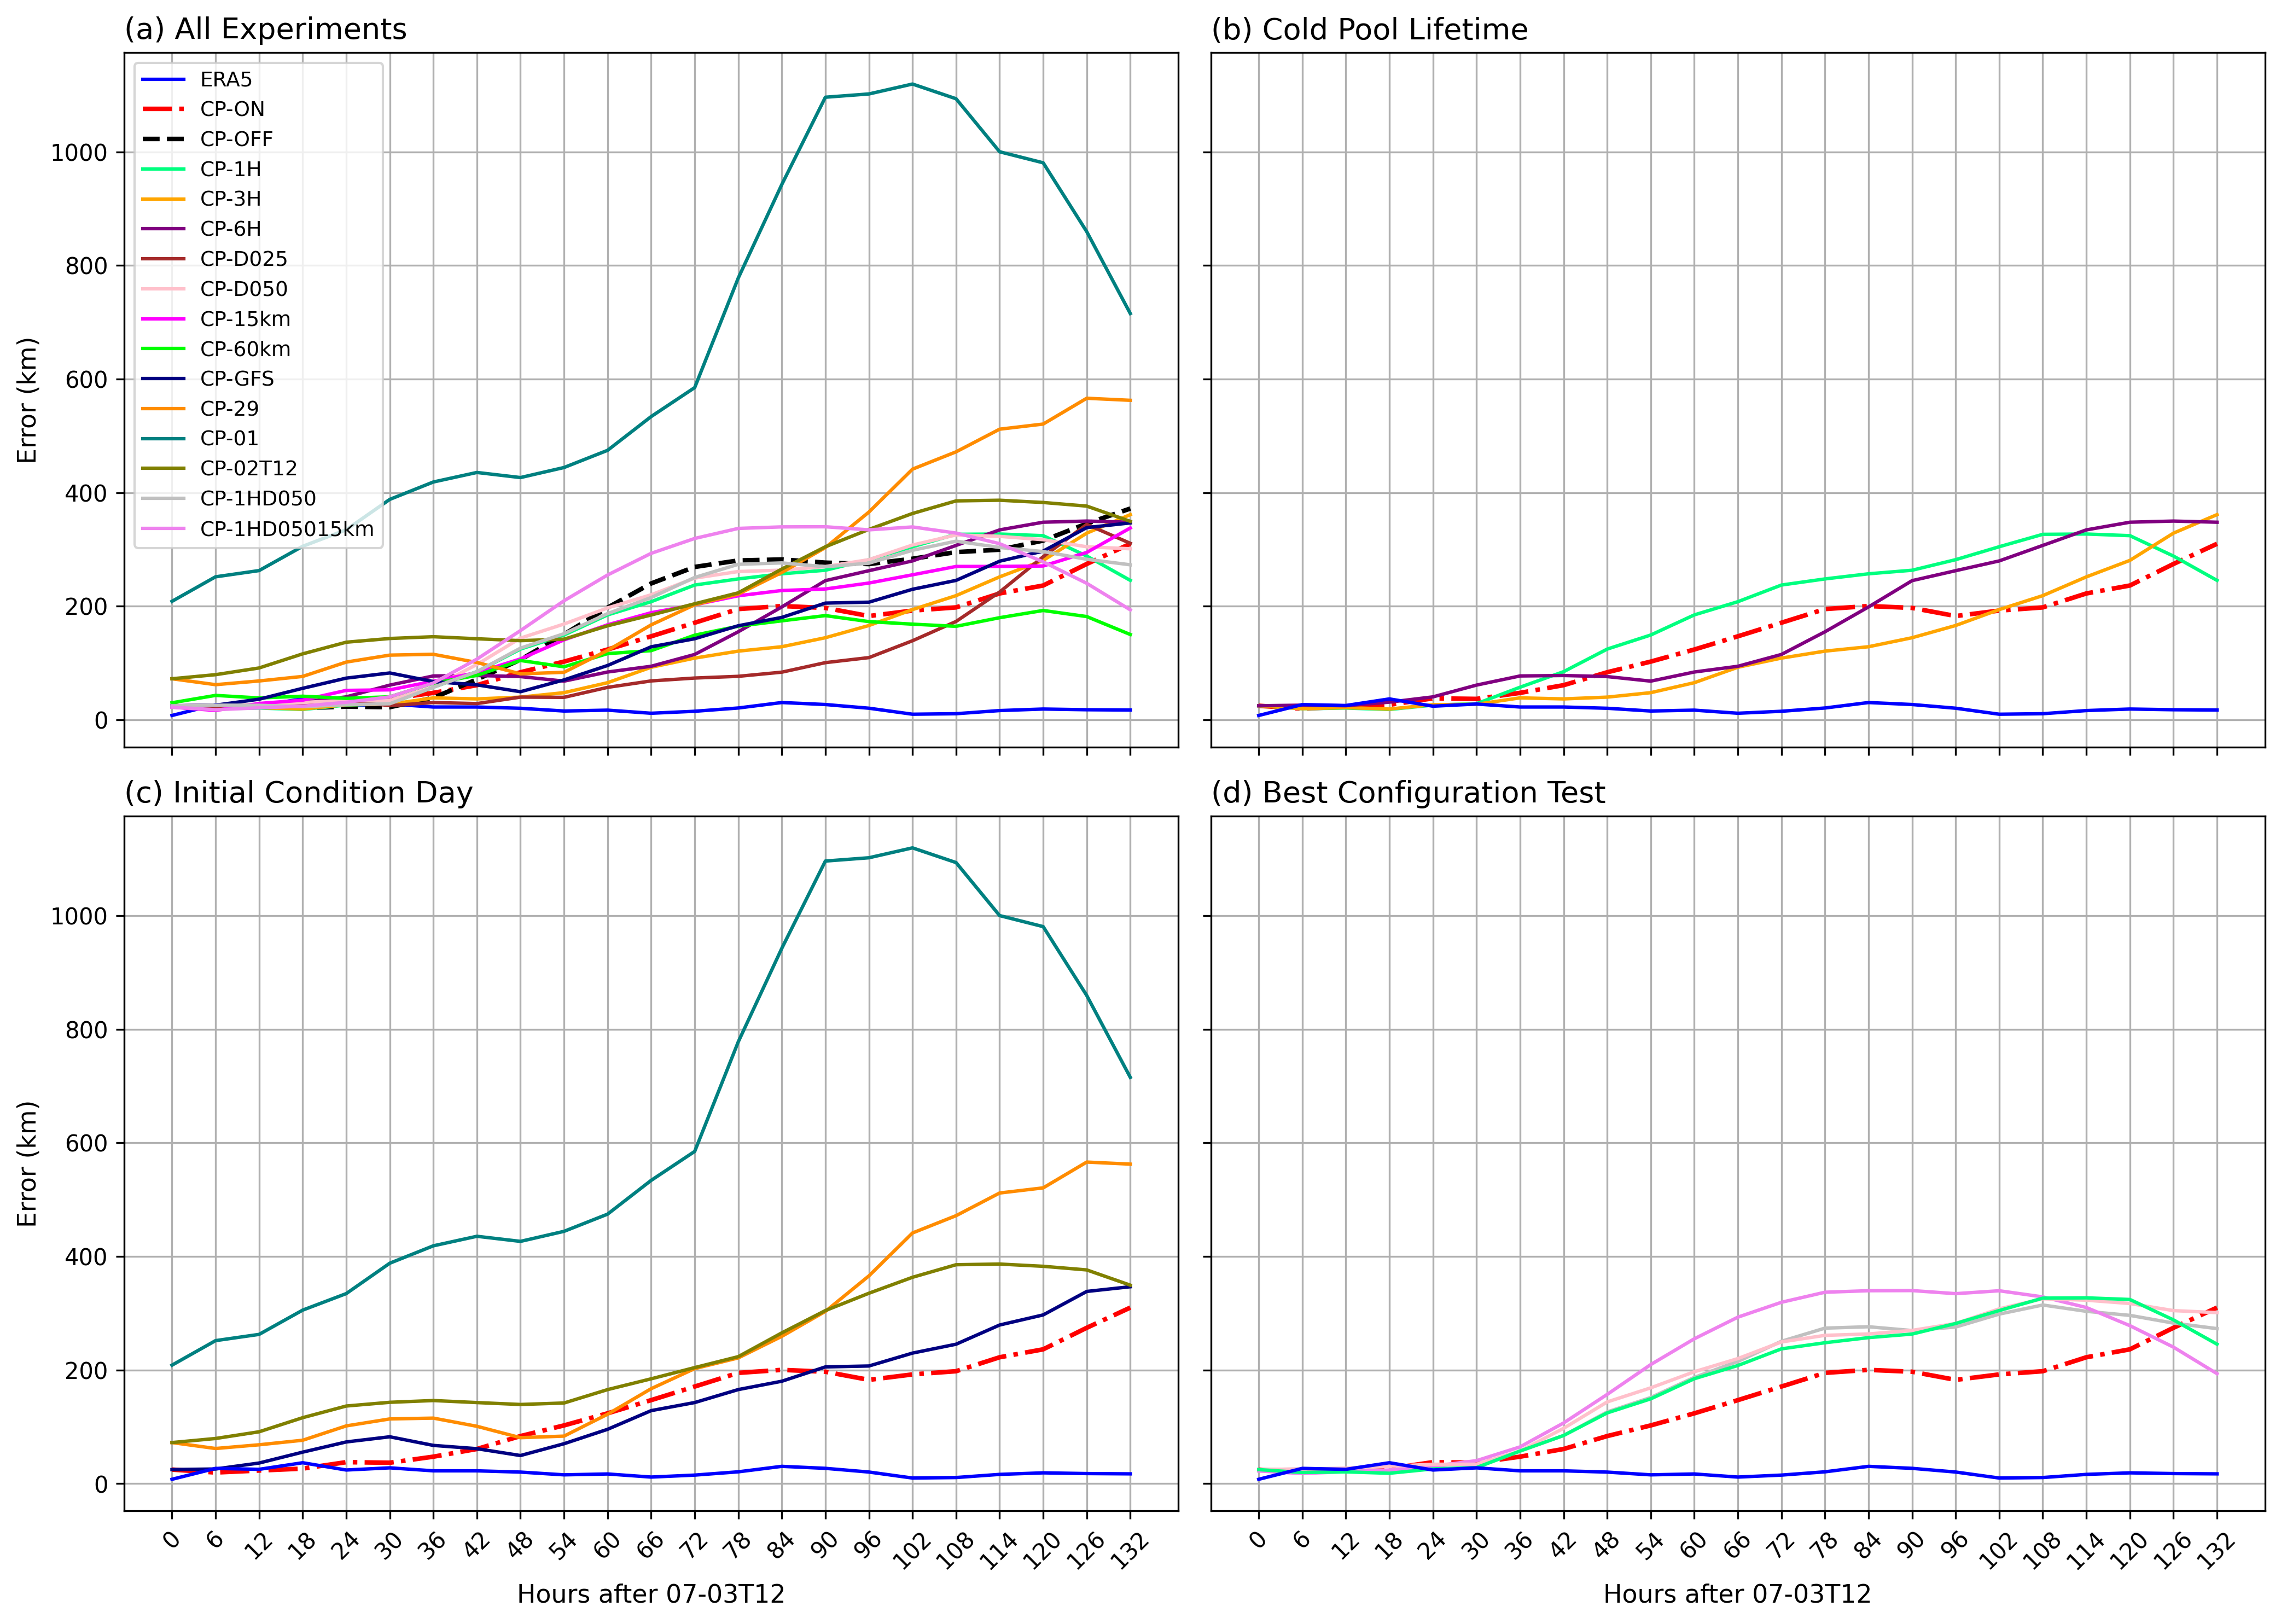
\includegraphics[width=\textwidth]{docs/figuras/findings/panel_2x2_error_comparison.png} % Substitua pelo caminho e extensão correta
    \vspace{0.5em}
    
    Source: Made by the author (2025). % Fonte abaixo da imagem
    \label{fig:panel_errors_before} % Label para referenciar no texto
\end{figure}

\pagebreak

It can be confirmed that CP-01 deviates significantly from the expected trajectory. Additionally, CP-6H offer limited discussion, as it is quite similar to the other experiments within their group. In Figure~\ref{fig:panel_errors_before} (d), CP-1HD05015km does not show a significant improvement and will consequently be withdrawn. We will retain CP-1HD050 to seek the effects related to this configuration in the context of other aspects of tropical cyclones.

To summarize the experiments we intend to keep, a new table has been created, similar to Table~\ref{tab:experiments_long}.

\pagebreak

\begin{center}
\captionof{table}{Selected Experiments} \label{tab:selected_experiments}
\end{center}

\begin{longtable}{m{3cm} m{8cm} m{3.5cm}}
\textbf{Experiment} & \textbf{Description} & \textbf{ID} \\
\hline
\endfirsthead

\textbf{Experiment} & \textbf{Description} & \textbf{ID} \\
\hline
\endhead

\multicolumn{3}{r}{\textit{Table continued on next page}} \\
\endfoot

\hline
\endlastfoot

Cold Pool Effect & Turn on and off the cold pool parameterization scheme & \makecell[l]{CP-ON\\CP-OFF (Control)} \\
\hline
Initial Condition & Compares the effect of two initial conditions, June 29, July 2nd (noon), and July 3rd. Tested with 1st July. & \makecell[l]{CP-29\\CP-02T12\\CP-03 (Control)} \\
\hline
Cold Pool Lifetime & Compares the effect of cold pool lifetime being 1h, 2h (default), 3h, and 6h & \makecell[l]{CP-1H\\CP-2H (Control)\\CP-3H} \\
\hline
Maximum Downdraft Height & Compares the effect of the maximum downdraft height, being 0.25, 0.35, and 0.50 & \makecell[l]{CP-D025\\CP-D035 (Control)\\CP-D050} \\
\hline
Resolution Experiment & Evaluates the resolution effect on the results, degrading it into 60 km and enhancing it into 15 km & \makecell[l]{CP-15km\\CP-30km (Control)\\CP-60km} \\
\hline
Type of Initial Condition & Changes the type of initial condition to be from the GFS model & \makecell[l]{CP-ERA5 (Control)\\CP-GFS} \\
\hline
Best Configuration Test & A run with two changes inside the cold pool parameters & \makecell[l]{CP-1HD050} \\
\end{longtable}

\begin{center}
\textit{Source: Made by the author, 2025.}
\end{center}

In the following subsection we will continue the results now keeping in mind the experiments listed at Table~\ref{tab:selected_experiments}.

%%%%%%%%%%%%%%%%%%%%%%%%%%%%%%%%%%%%%%%%%%

\subsection{Trajectory}


All trajectories are displayed in the Figure~\ref{fig:all_tracks_selected}. The trajectories of each group of the Table~\ref{tab:selected_experiments} can be found at Appendix ().

\begin{figure}[!ht]
    \centering
    \caption{All tracks with selected experiments from Table~\ref{tab:selected_experiments}} % Título acima da figura
    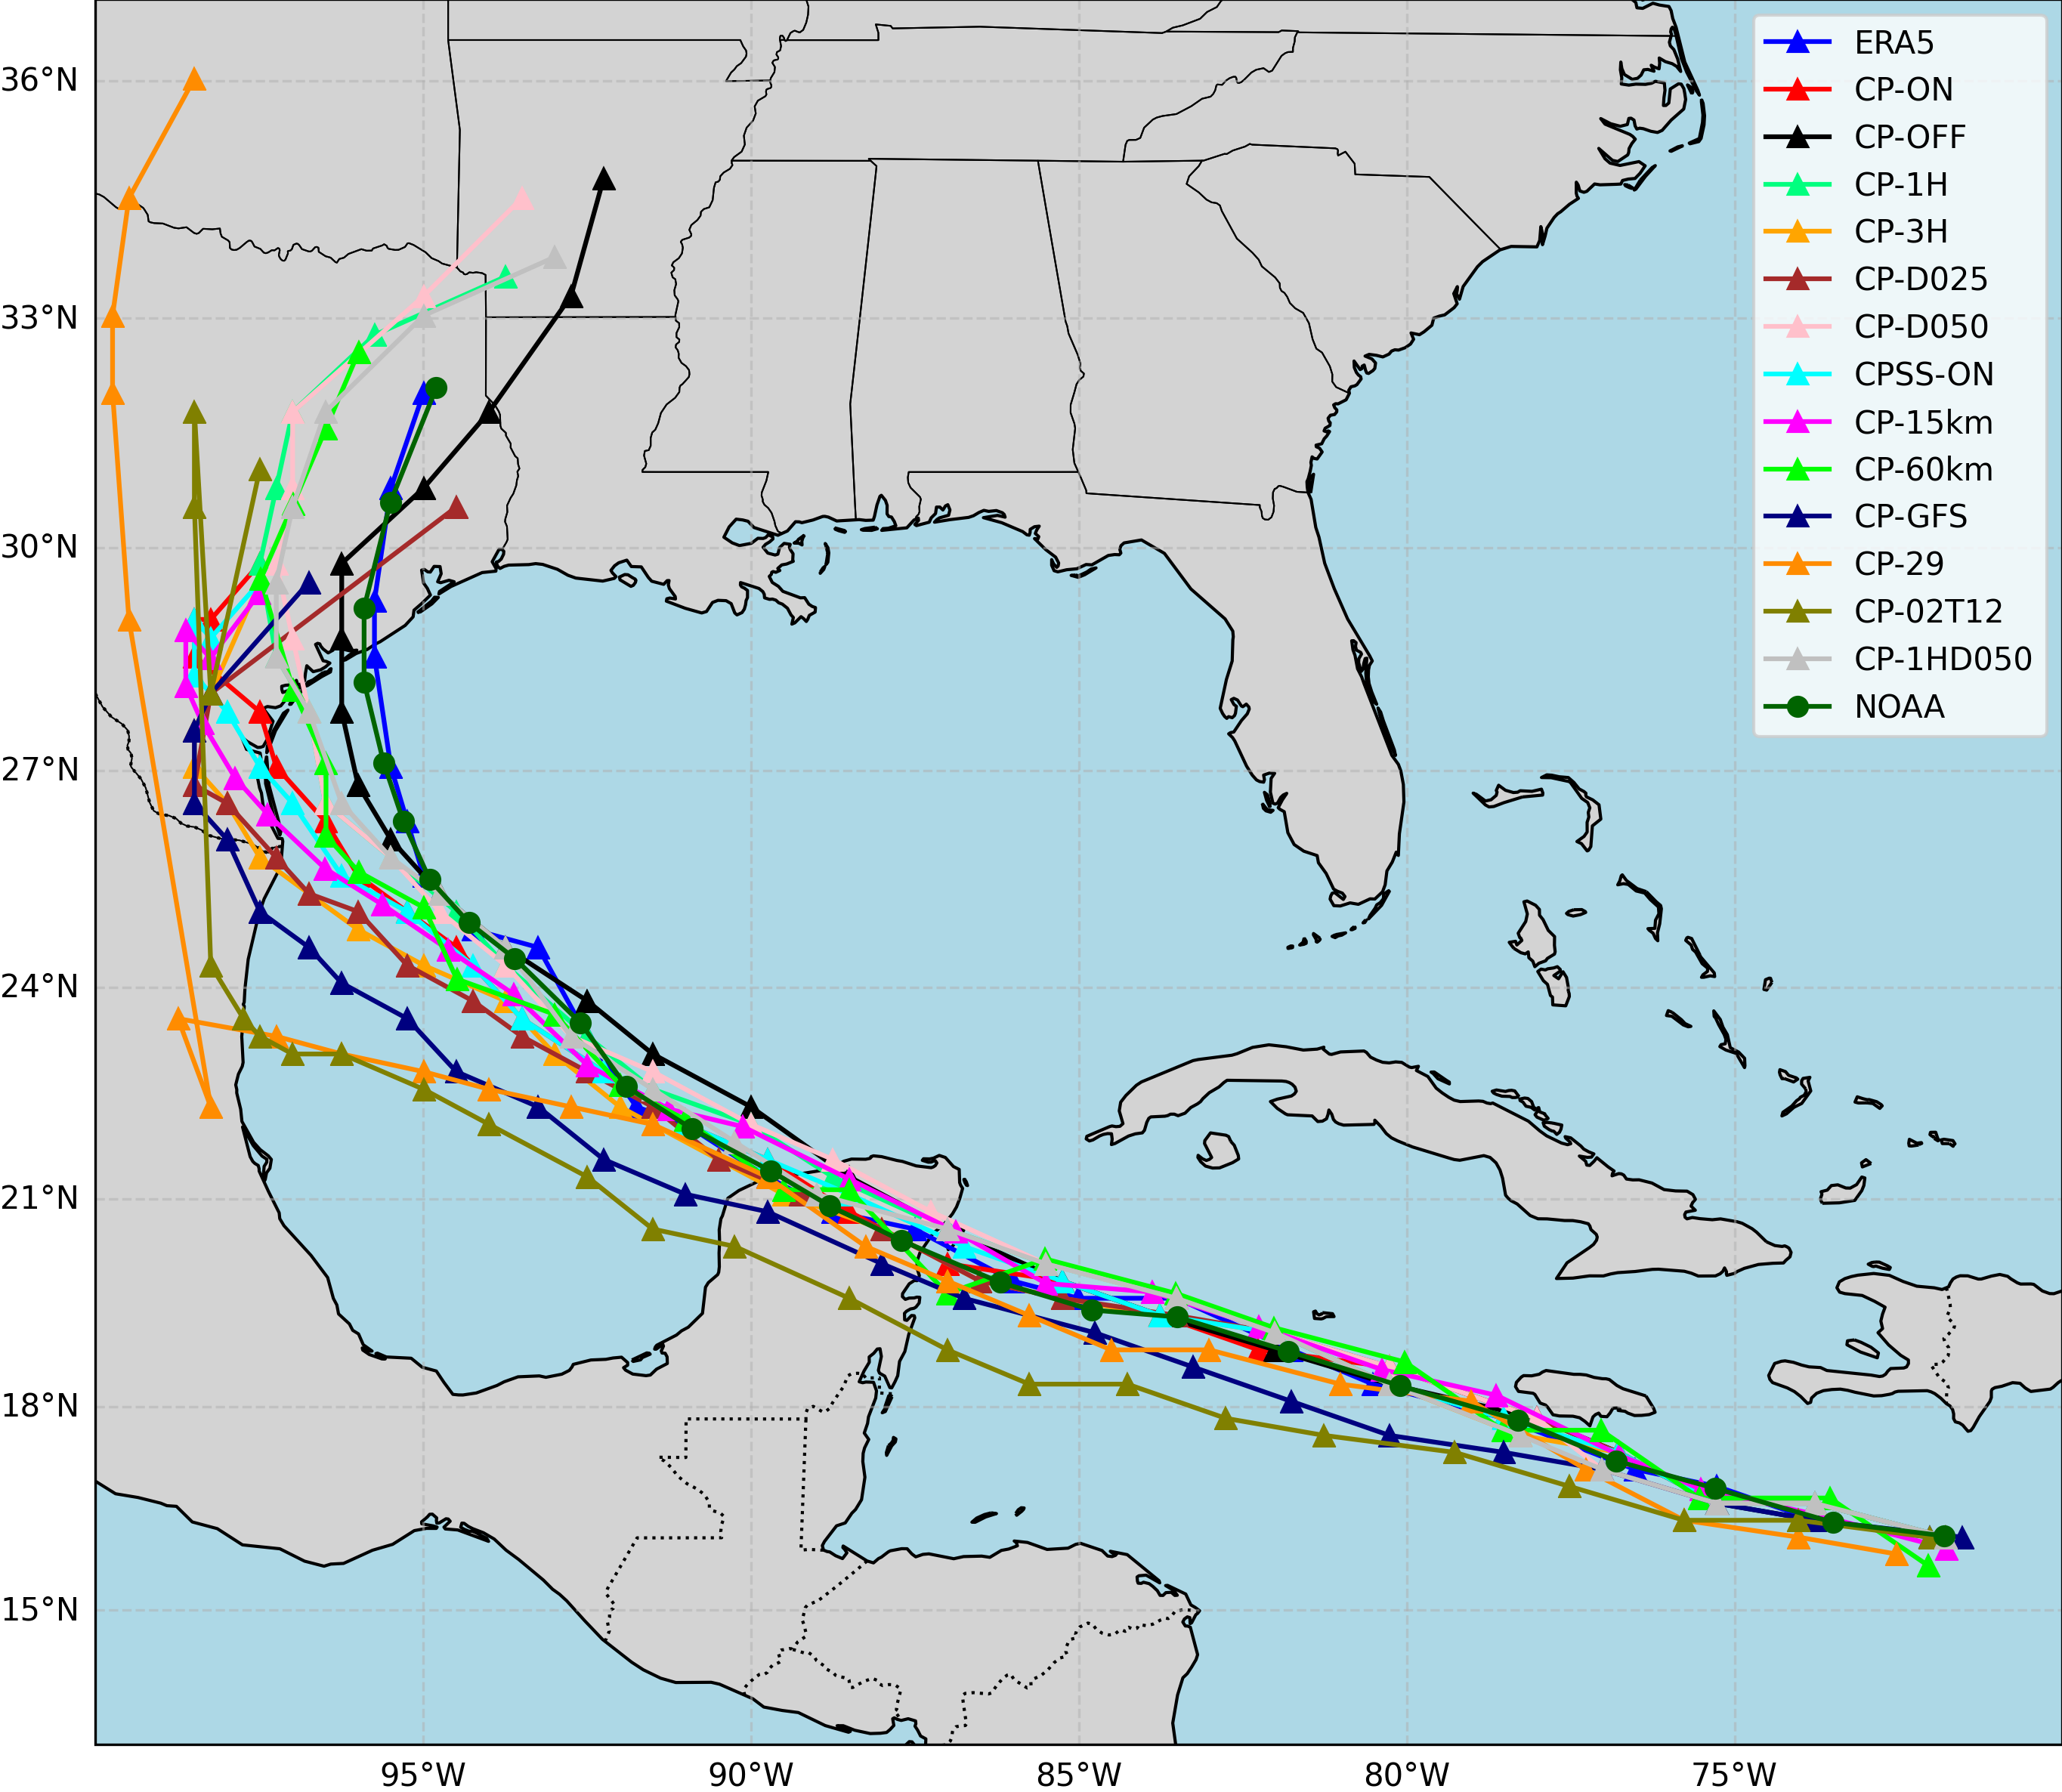
\includegraphics[width=\textwidth]{docs/figuras/findings/ALL_tracks_filtered.png} 
    \vspace{0.5em}
    
    Source: Made by the author (2025). % Fonte abaixo da imagem
    \label{fig:all_tracks_selected} % Label para referenciar no texto
\end{figure}

\subsection{Intensity}




\subsection{Rainfall}

\subsubsection{Pattern and spatial rainfall distribution}

\subsubsection{Rainfall mean and overall distribution}

\subsubsection{MONAN performance at forecasting rainfall}

\subsection{Discussion of key outcomes}

